\section{Experiments}
\label{sec:experiments}

Our experiments answer three questions: (1) does the first-layer phase formula
reconstruct a real model's QK score; (2) does the resulting state divergence
causally affect the output; and (3) does a mechanism-derived semantic proposal
improve retrieval at a matched sparse budget?  The first two were reported in
\cref{sec:mechanism}; this section focuses on the method evaluation and its
current limits.

\subsection{Protocol}

\paragraph{Model and contexts.}
We use Qwen3-8B with NF4 weights and BF16 computation for the held-out method
evaluation.  Filler-body targets are 8,192, 16,384, 32,768, and 65,536 tokens;
after the chat wrapper and query suffix, exact prompt lengths are 8,284, 16,476,
32,860, and 65,628 tokens.  The model's configured native window is 40,960;
the 64K condition uses dynamic YaRN scaling, while the first three conditions
remain within that window.
Results from native and position-extended conditions are always identified.

\paragraph{Data.}
Each example samples three ordinary English words that are stable single
tokens in the tokenizer and absent from the filler corpus.  Two lines encode a
verified chain $c_0\rightarrow c_1\rightarrow c_2$ near token 256.  Randomized
English paragraphs fill the remaining body, and a fixed concise query at the
end asks for the two-step result.  The gold output is the single token $c_2$.
Seeds 0--7 were used for development; all reported main results use frozen
seeds 32--55, i.e., 24 unseen examples at every length and 96 paired
length--example points.

\paragraph{Baselines.}
\textbf{Full RoPE} is the unmodified dense attention.  \textbf{post-RoPE
Top-2\%} computes all standard logits and retains the exact highest 2\% per
layer and query head.  It is an exact score-based sparse reference whose
selection itself costs a full score scan.  \textbf{\methodpost} uses the same
2\% budget, 128 local tokens, and 16 sinks, but proposes the remaining remote
tokens with \cref{eq:content-score} before exact post-RoPE consumption.

\paragraph{Metrics and statistics.}
We report first-token accuracy and \GoldPPL, computed by averaging gold NLL and
then exponentiating.  Candidate recall is the fraction of gold evidence tokens
selected, averaged over layer--head rows.  Chain completion is the fraction of
rows that select at least one token from both evidence lines.  Evidence mass is
the post-softmax mass on gold spans.  Confidence intervals use 20,000 paired
bootstrap resamples over seeds; heads and layers are never treated as
independent samples.

\subsection{Main results}

\begin{figure}[t]
  \centering
  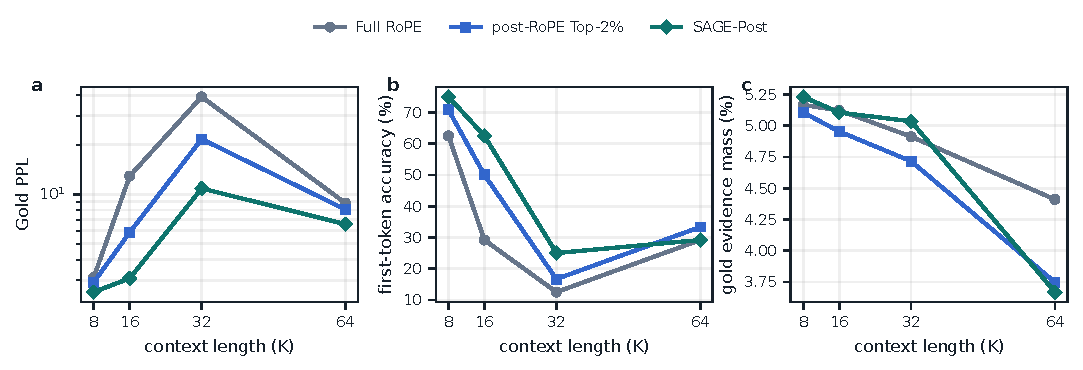
\includegraphics[width=\linewidth]{figures/heldout_results.pdf}
  \caption{Held-out two-hop results (24 seeds per length).  Lower is better for
  \GoldPPL; higher is better otherwise.  SAGE-Post is strongest at 16K and
  32K.  Non-monotonic curves are expected under the phase-sensitive account
  and caution against summarizing the problem as simple distance decay.}
  \label{fig:heldout}
\end{figure}

\begin{table}[t]
  \caption{Held-out gold-answer quality.  Accuracy is exact first-token
  accuracy.  All methods use the same prompts; sparse methods retain 2\% of
  tokens per layer and query head.}
  \label{tab:quality}
  \centering
  \small
  \setlength{\tabcolsep}{4.1pt}
  \begin{tabular}{r rr rr rr}
    \toprule
    & \multicolumn{2}{c}{Full RoPE}
    & \multicolumn{2}{c}{post-RoPE Top-2\%}
    & \multicolumn{2}{c}{\methodpost}\\
    \cmidrule(lr){2-3}\cmidrule(lr){4-5}\cmidrule(lr){6-7}
    Length & PPL & Acc. & PPL & Acc. & PPL & Acc.\\
    \midrule
    8K  & 3.120  & 62.5 & 2.914  & 70.8 & \textbf{2.541}  & \textbf{75.0}\\
    16K & 12.885 & 29.2 & 5.858  & 50.0 & \textbf{3.080}  & \textbf{62.5}\\
    32K & 39.079 & 12.5 & 21.636 & 16.7 & \textbf{10.840} & \textbf{25.0}\\
    64K & 8.823  & 29.2 & 8.063  & \textbf{33.3} & \textbf{6.573} & 29.2\\
    \bottomrule
  \end{tabular}
\end{table}

\methodpost improves \GoldPPL over Full at all four point estimates and
first-token accuracy at three of four lengths (\cref{tab:quality}).  With equal
weight per length--seed pair, geometric \GoldPPL falls from 10.851 to 4.859,
and mean accuracy rises from 33.3\% to 47.9\%.  The full-attention comparison
is statistically significant at 8K, 16K, and 32K; at 64K the NLL interval is
$[-0.615,0.004]$ and does not establish a reliable gain.

The stricter comparison is exact post-RoPE Top-2\%, which isolates candidate
choice at the same budget.  At 16K, \methodpost reduces mean NLL by 0.643
(95\% CI $[-0.973,-0.342]$), corresponding to a $1.90\times$ geometric
quality ratio.  At 32K the reduction is 0.691
($[-1.035,-0.308]$), or $2.00\times$.  The 8K and 64K intervals cross zero.
Thus the current evidence supports a long-range compensation region, not an
unconditional replacement for post-RoPE selection.

\begin{table}[t]
  \caption{Candidate and attention diagnostics.  Rec. is gold evidence-token
  recall; Chain is the fraction of layer--head rows hitting both evidence
  lines; Mass is post-softmax gold evidence mass.}
  \label{tab:mechanism-metrics}
  \centering
  \small
  \setlength{\tabcolsep}{4.4pt}
  \begin{tabular}{r l rrr}
    \toprule
    Length & Method & Rec. (\%) & Chain (\%) & Mass (\%)\\
    \midrule
    \multirow{2}{*}{8K}
      & post-RoPE Top-2\% & 32.10 & 64.48 & 5.11\\
      & \methodpost        & 14.07 & 55.72 & 5.23\\
    \midrule
    \multirow{2}{*}{16K}
      & post-RoPE Top-2\% & 35.64 & 60.00 & 4.95\\
      & \methodpost        & \textbf{40.50} & \textbf{78.56} & \textbf{5.11}\\
    \midrule
    \multirow{2}{*}{32K}
      & post-RoPE Top-2\% & 38.98 & 60.59 & 4.72\\
      & \methodpost        & \textbf{46.71} & \textbf{80.05} & \textbf{5.04}\\
    \midrule
    \multirow{2}{*}{64K}
      & post-RoPE Top-2\% & 35.12 & 54.92 & \textbf{3.75}\\
      & \methodpost        & \textbf{44.45} & \textbf{78.16} & 3.67\\
    \bottomrule
  \end{tabular}
\end{table}

The internal metrics localize the benefit.  At 16K and 32K, where paired NLL
improves reliably, \methodpost also increases token recall, two-line chain
completion, and evidence mass (\cref{tab:mechanism-metrics}).  At 64K it
improves recall and chain completion but not mass or accuracy, indicating that
candidate recovery alone is insufficient when selected evidence still
receives weak post-RoPE weight.  At 8K, lower token recall coexists with better
PPL, showing that undifferentiated span recall is not a complete proxy for
answer-relevant head behavior.  These exceptions are useful: they argue for a
distance- and head-aware gate rather than a universal semantic branch.

\subsection{Ablations and missing validation}

Calibrated pre/post score mixtures and mass-preserving remote reranking improve
the aggregate pilot point estimate beyond \methodpost, but they modify the
pretrained attention logits and are therefore kept as appendix ablations.  We
select \methodpost as the primary result because it provides the cleanest
causal attribution.

The present evaluation is intentionally narrow.  \todoexp{Add RULER and a
natural multi-hop benchmark under the same paired protocol.}
\todoexp{Replicate on at least one native long-context RoPE architecture.}
\todoexp{Measure short-context language-model PPL and local order tasks.}
\todoexp{Replace the exact semantic proposal scan with an approximate index and
measure end-to-end systems cost.}  Until these tests are complete, our method
claim is limited to controlled long-range evidence retrieval.
